\section{Background}
\label{sec:synthesis}


In this section we define Assume-Guarantee contracts (Sect.~\ref{sec:pre}),
describe the validity-guided approach we take towards synthesizing
implementations (Sect.~\ref{sec:synth}),
and finally illustrate how it works using the popular cinderella-stepmother
game (Sect.~\ref{sec:example}).
%Finally, we enrich our formal definitions with an informal proof of the
%algorithm's correctness in terms of the successfully synthesized
%implementations.

\subsection{Assume-Guarantee Contracts}
\label{sec:pre}

For the purposes of this paper, we focus our interest in a mainstream variation
for representing system requirements, using an \textit{Assume-Guarantee
Contract}. Requirements in this format contain two main types of constraints.
The \emph{assumptions} of the contract restrict the possible inputs that the
environment can provide to the system, while the \emph{guarantees} are used to
describe what is considered a safe reaction of the system to the outside world.

A simple example is the contract with assumption $A = \{x\neq
y\}$ and guarantee $G = \{x \leq y \Rightarrow z =
\textit{true}, x \geq y \Rightarrow z = \textit{false}\}$. Variables
$x$ and $y$ are the designated inputs while $z$ is the output. This is a
well-defined contract, since by the assumption $A$, it is always the case that
$x \neq y$, therefore at least one implementation exists, which, for example
sets $z$ to true if $x < y$ and false otherwise. An alternative
valid implementation could set $z$ to false if $x > y$, and true otherwise. The
proof of existence of such an implementation is the main concept behind the
\emph{realizability} problem, while the automated construction of a witness
implementation is the main focus of \emph{program synthesis}.


It is apparent that the example contract above is therefore \emph{realizable},
and an efficient synthesis procedure would be capable of providing at least one
implementation. Nevertheless, it is important to consider a variation of the
example, where $A = \varnothing$. This is a practical case of an
\emph{unrealizable} contract, as there is no feasible implementation that can
correctly react to the environment assigning values to $x$ and $y$, such that
$x = y$.

\subsection{Formal Representation}
\label{sec:formals}
We use two disjoint sets, $state$ and $inputs$, to describe a system.
A straightforward and intuitive way to represent an \emph{implementation} is by
defining a \emph{transition system}, composed of an initial state
predicate $I(s)$ of type $state \to bool$, as well as a transition relation
$T(s,i,s')$ of type $state \to inputs \to state \to bool$.

Combining the above, we represent an Assume-Guarantee (AG) contract using a set
of \emph{assumptions}, $A: state \rightarrow inputs \rightarrow bool$,
and a set of \emph{guarantees} $G$. The latter is further decomposed into two
distinct subsets $G_I: state \rightarrow bool$ and $G_T: state \rightarrow
inputs \rightarrow state \rightarrow bool$. $G_I$ defines the set of valid
initial states, and $G_T$ contains constraints that need to be satisfied in
every transition between two states. An important note at this point is that we
we do not make any distinction between internal state variables and outputs in the
formalism. This alone allows us to use state variables to (in some cases)
simplify specification of guarantees, since we do not expect a contract
to be always defined over all variables in the transition system.

Consequently, we can formally define a realizable contract, as one for which any
preceeding state $s$ can take a transition into a new state $s'$ that satisfies
the guarantees, assuming valid inputs. For a system to be ever-reactive, these
new states $s'$ should be further usable as preceeding states in a future
transition. States like $s$ and $s'$ are defined as being \textit{viable}, if
and only if:

\begin{equation}
\forall s,i.~ A(s, i) \land \viable(s) \Rightarrow \exists s'.~ G_T(s, i,s')
\land \viable(s')
\label{eq:viable}
\end{equation}

A necessary condition, finally, is that the set of viable states
intersects with the set of initial states. As such, to conclude that a contract
is realizable, we require that

\begin{equation}
\viable(s) \land G_I(s) \neq \varnothing
\label{eq:nonempty}
\end{equation}

The intuition behind our proposed algorithm in this paper relies on the
discovery of a greatest fixpoint that only contains viable states.

\subsection{\textit{AE-VAL}}
\label{sec:aeval}

\begin{figure}[!t]
\centering
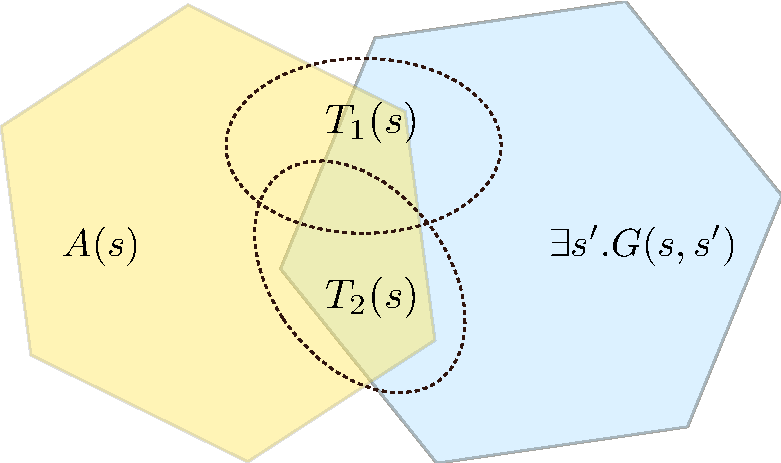
\includegraphics[width=2.5in]{aeval_invalid}
\caption{Region of validity computed for an example requiring \aeval to iterate two times.}
\label{fg:aeval}
\end{figure}

\aeval~\cite{fedyukovich2015automated} is an algorithm to decide validity and extract Skolem functions.
It takes as input a formula of the form $\forall s \,.\,  A(s) \Rightarrow \exists s' . G(s,s')$, 
where $A(s)$ has only existential\andreas{you meant universal here, right?} quantifiers, and $G(s,s')$ is quantifier-free.
%
While deciding the validity, \aeval iteratively enumerates models of $A(s) \land G (s, s')$ and groups them into a set of partitions $\{P_i(s)\}$, such that each $P_i(s) \Rightarrow \exists s' . G (s, s')$.
We say that after $n$ iterations, \aeval establishes a formula $R_n(s) \eqdef \bigvee_{i=1}^n P_i(s)$ which is by definition an under-approximation of $\exists s' . G (s, s')$.

If after $n$ iterations, it happens that $A(s) \Rightarrow R_n(s)$ then $\forall s \,.\,  A(s) \Rightarrow \exists s' . G(s,s')$ is valid, and \aeval generates a Skolem function as described in~\cite{katis2016synthesis}.
Alternatively, if $A(s) \land  G (s, s') \land \neg{R_n (s, s')}$ is unsatisfiable, then $A(s) \land \neg G (s, s')$ is satisfiable, or equivalently $\forall s \,.\,  A(s) \Rightarrow \exists s' . G(s,s')$ is invalid (see an example in Figure~\ref{fg:aeval}).
In both cases, we say that $A(s) \land R_n(s)$ is a \emph{region of validity}, meaning that $\forall s \,.\,  A(s) \land R_n(s) \Rightarrow \exists s' . G(s,s')$ is valid by construction.

\begin{lemma}
If formula $\forall s \,.\,  A(s) \Rightarrow \exists s' . G(s,s')$ is invalid, and $A(s) \land R_n(s)$ is the region of validity, then there is no other formula $S(s)$ such that $A(s) \land R_n(s) \Rightarrow S(s)$ and $\forall s \,.\,  S(s) \Rightarrow \exists s' . G(s,s')$.

\label{lem:subset}
\end{lemma}


\section{Validity-Guided Synthesis from Assume-Guarantee Contracts}
\label{sec:synth}

\begin{algorithm}[!t]
\footnotesize
\caption{\jsynvg (A : assumptions, G : guarantees)}\label{alg:synthesis}
\begin{algorithmic}[1]
%\Procedure{\jsynvg}{A : assumptions, G : guarantees}
	\State $F(s) \gets true$;\Comment{Fixpoint of viable states}
	\While{true}
		\State $\phi \gets \forall s,i. F(s) \land A(s,i) \Rightarrow \exists s'.G_{T}(s,i,s') \land F(s')$;
		\State $\tuple{\skolems, \subs} \gets \aeval(\phi)$;
		\If{$\isValid(\phi)$}
			\If{$G_{I}(s) \land F(s) \neq false$}
				\Return $\tuple{\realizable, \skolems}$;
			\Else{\Comment{Empty set of initial states}}
		 		\Return $\tuple{\unrealizable, \varnothing}$;
				\State
		 	\EndIf
		\Else{\Comment{Extract region of validity $Q(s,i)$}}
			\State $Q(s,i) \gets \subs$;
			\If{$Q(s,i) = false$}
				\Return $\tuple{\unrealizable, \varnothing}$;
				\State
			\EndIf
			\State $\phi' \gets \forall s. F(s) \Rightarrow \exists i. A(s,i) \land \lnot
			Q(s,i)$;
			\State $\tuple{\skolems', \subs'}\gets \aeval(\phi')$;
			\If{$(\isValid(\phi'))$}\Comment{If $Q(s,i)$ contains only unsafe states}
			        \State\Comment{Extract witnessing cex}
				\Return $\tuple{\unrealizable, \skolems'}$;
				\State
			\Else{}
				\State $W(s) \gets \subs'$;
				\State $F(s) = F(s) \land \lnot W(s)$;\Comment{Refine candidate fixpoint}
			\EndIf
		\EndIf
	\EndWhile
%\EndProcedure
\end{algorithmic}
\end{algorithm}

The main contribution presented in this paper, is a novel idea that effectively
uses the information provided by \textit{regions of validity} to compute a
greatest fixpoint of safe states. In our context, this fixpoint is not only
usable as a proof to the realizability of a specification, but also leads to the
construction of a witness that can be translated with a straightforward process
into a functional and efficient implementation.

\grigory{Please, add references to lines from the text}

Algorithm~\ref{alg:synthesis} shows this validity-guided technique, which we
named \jsynvg.
We initialize the process by defining the fixpoint $F(s)$ to be equal to $true$.
Eventually, the algorithm attempts to converge to such a fixpoint $F(s)$ that
only contains viable states, considering Equation~\ref{eq:viable}
and~\ref{eq:nonempty}.
We therefore construct the formula $\phi = \forall s,i. F(s) \land A(s,i)
\Rightarrow \exists s'.
			G_{T}(s,i,s') \land F(s')$, and provide it as an input to \aeval, an efficient
Skolemizer for $\forall\exists$ formulas. \aeval is particularly focused on
determining the validity of $\phi$. If the formula is valid, then a witness
\textit{Skolem} is constructed, containing valid assignments to the
existentially quantified variables of $\phi$. In the context of viability, this
witness is capable of providing viable states that can be used as a safe
reaction, considering the precedence of a viable state and an input that
satisfies the assumptions.

If $\phi$ is not true for every possible assignment of the universally
quantified variables, \aeval provides an exact subset of $F(s) \land A(s,i)$, namely
$Q(s,i)$, which, if plugged in the original left-hand side of $\phi$, makes the
resulting formula valid. We will refer to such subsets as \textit{regions of
validity}.
\grigory{now, the definition is in Sect.~\ref{sec:aeval}.}

At this point, one could falsely assume that replacing $F(s) \land A(s,i)$ with
$Q(s,i)$ is sufficient to solve our problem, and use the resulting witness as a
candidate implementation. This is not the case however, as $Q(s,i)$ is a subset
of both state and input variables. As such, it may contain further constraints
over the contract's inputs. This would lead to implementations that only
consider a subset of the original assumptions of the contract, with no
pre-defined strategy for the rest of the originally valid inputs.
Fortunately, we can exploit \aeval's capability of providing regions of validity
towards eliminating this issue.

The main concept to properly refine $F(s)$, is to extract a region of validity
that only involves constraints over state variables. To achieve this, we ask for
the validity of the formula $\phi' = \forall s. F(s) \Rightarrow \exists
i. A(s,i) \land \lnot Q(s,i)$. If $\phi'$ is a valid formula, then for any
assignment of the state variables $s$, we have a valid input (i.e. that
satisfies the assumptions), for which the states are taken outside of the region
of validity $Q(s,i)$. This is a case of an unrealizable contract, as no state is
safe in this context. On the other hand, if $\phi'$ is not valid, \aeval computes
a new region of validity, namely $W(s)$. The new region is a strict subset of
$F(s)$, is described using constraints over state variables only, and entails
the existence of unsafe states in $F(s)$, considering valid inputs.

Having this new region of validity, we can finally refine $F(s)$, by conjucting
to it the negation of $W(s)$. Despite the fact that we now have a refined
candidate fixpoint, we are not yet done, as $\lnot W(s)$ is not an exact region
of validity, with respect to $Q(s,i)$. As such there might still be states in
$Q(s,i)$ that are not covered by $\lnot W(s)$. Therefore, we reiterate the
process by repeating the top-level \aeval query, with $F(s) = F(s) \land \lnot
W(s)$. Eventually, we either reach a greatest fixpoint $F(s)$ that effectively
describes the set of viable states, or reach the case where $F(s) = false$, and
declare our contract to be unrealizable.

\aeval's effectiveness in providing witnesses to the
satisfiability of $\forall\exists$ formulas is also exploited in terms of the
tool providing concrete counterexamples to unrealizable contracts, using line 19
in Algorithm~\ref{alg:synthesis}. In this particular case, if $\phi'$ is a valid
formula, we can extract a witness that can be essentially used as a test case to
demonstrate the specification's unrealizability. The witness contains
certain assignments to input variables, for which the condition of viability does not
hold, for any state. We leave the specifics regarding the meaning and usability
of such counterexamples as potential future work.

\subsection{Soundness}

From the previous, it is straightforward to show that
Algorithm~\ref{alg:synthesis} is complete, since it either terminates by
constructing a fixpoint, or when the computed region of validity is the empty
set \textit{false}. To prove its soundness regarding results, we require that
the algorithm always computes a fixpoint, containing only state variable assignments that lead to the satisfiability of $\forall\exists$
formulas following the form of Equation~\ref{eq:viable}. To achieve this, we
use the fixed point theorem that was first stated by Alfred Tarski~\cite{tarski1955lattice}.

\begin{lemma} Consider the system
$\mathfrak{U} = \tuple{S, T}$. With $S$, we denote the set of
subsets of the orignal state space, such that each subset contains assignments that lead to the
satisfiability of Equation~\ref{eq:viable}. By $T$, we refer to the
transition relation between any two states, that establishes a partial order
on $S$. Then $\mathfrak{U}$ is a complete lattice, where every subset $B \subseteq
S$ has a greatest lower bound  $\glb = \cap B$  and a least upper
bound $\lub = \cup B$.
\label{lem:lattice}
\end{lemma}
\begin{proof}
Considering the partial order that is established by T, it is straightforward
to show that all subsets $B$ of $S$ contain a \glb and a \lub. These
are respectively, the states which have no preceeding state in $B$ other than
possible ones in the \glb, and the states from which we take a transition into
a new state that's either in the \lub, or outside of $B$. For the special case
where $B = S$, we have that $\glb = false$ and $\lub = true$.
\end{proof}

\begin{lemma} Algorithm~\ref{alg:synthesis} is a monotonic function on $S$ to
$S$.
\label{lem:monotonicity}
\end{lemma}
\begin{proof}
The algorithm recursively reduces $S$, attempting to reach a fixed point
at which $S$ only contains state assignments that lead to the satisfiability of
Equation~\ref{eq:viable}. As such, it can be considered as an isotone function
$f$, where, for every pair $(B,A)$ with $B \subseteq A \subseteq S$, we have that
$f(B) \subseteq f(A)$.
\end{proof}

\begin{theorem}[Soundness of Fixpoint]
The set $P$ of all fixpoints in Algorithm~\ref{alg:synthesis} is non
empty, and the system $\tuple{P, T}$ is a complete lattice.
\label{thm:fixpoint}
\end{theorem}
\begin{proof}
The proof relies on Tarski's first theorem on fixed
points~\cite{tarski1955lattice}.
Considering Lemmas~\ref{lem:lattice} and~\ref{lem:monotonicity}, we satisfy the first two
conditions of Tarski's theorem. When the specification is realizable, a
fixpoint is reached by Algorithm~\ref{alg:synthesis}, since each consecutive
attempt to further refine $F(s)$ results in the same set. On the other hand, if
the specification is unrealizable, the algorithm returns the fixpoint $F(s) = false$. Therefore, the
set $P$ of all fixpoints in Algorithm~\ref{alg:synthesis} contains at least two
fixpoints.

Since all three conditions of Tarski's Fixed Point theorem are satisfied by our
solution, we can conclude that $P$ is a non empty set, while the system
$\tuple{P, T}$ is a complete lattice, as it contains a \lub, which is
the solution to a realizable contract, while $\glb = false$, and corresponds to
the solution for an unrealizable contract.
\end{proof}


\subsection{Example: The Cinderella-Stepmother Game}
\label{sec:example}

For the purposes of this paper, we will illustrate how the validity
guided-synthesis algorithm works, using a variation of the minimum-backlog
problem, the two player game between Cinderella and her wicked
Stepmother, first  expressed by Bodlaender \textit{et
al.}~\cite{bodlaender2012cinderella}.

The main objective for Cinderella (i.e. the reactive system) is to keep a
collection of buckets from overflowing with water. On the other hand,
Cinderella's Stepmother (i.e. the system's environment), attempts to fill the
buckets with water in such a manner that a bucket overflow must eventually
happen.
For the running example, we chose an instance of the game that has been
previously used in template-based synthesis~\cite{beyene2014constraint}. In this instance, the game is described
using five buckets, where each bucket can contain up to two units of water.
Cinderella has the option to empty two adjacent buckets at each of her turns,
while the Stepmother distributes one unit of water over all five buckets.

\begin{figure}[!t]
\centering
 \begin{Verbatim}[fontsize=\scriptsize]
const C = 2.0;

-- empty buckets e and e+1 each round
node game(i1,i2,i3,i4,i5: real; e: int)
	returns (guarantee: bool);
var
  b1, b2, b3, b4, b5 : real;
let
  assert i1 >= 0.0 and i2 >= 0.0 and
 	i3 >= 0.0 and i4 >= 0.0 and i5 >= 0.0;
  assert i1 + i2 + i3 + i4 + i5 = 1.0;

  b1 = 0.0 ->
       (if (e = 5 or e = 1) then i1 else (pre(b1) + i1)) ;
  b2 = 0.0 ->
       (if (e = 1 or e = 2) then i2 else (pre(b2) + i2)) ;
  b3 = 0.0 ->
       (if (e = 2 or e = 3) then i3 else (pre(b3) + i3)) ;
  b4 = 0.0 ->
       (if (e = 3 or e = 4) then i4 else (pre(b4) + i4)) ;
  b5 = 0.0 ->
       (if (e = 4 or e = 5) then i5 else (pre(b5) + i5)) ;

  guarantee = b1 <= C and b2 <= C and b3 <= C and
  	    b4 <= C and b5 <= C;

  --%REALIZABLE i1, i2, i3, i4, i5;
  --%PROPERTY guarantee;
tel;
 \end{Verbatim}
\caption{An Assume-Guarantee contract for the Cinderella-Stepmother game}
\label{fg:cind}
\end{figure}

Figure~\ref{fg:cind} shows one possible interpretation of a contract designed
for the aforementioned instance of the Cinderella-Stepmother game. The contract
is expressed using Lustre~\cite{lustrev6}, a language
that has been extensively used for specification as well as implementation of
safety-critical systems, and is the kernel language in SCADE, a popular tool in
model-based development. The contract is defined as a Lustre node, with a global
constant $C$ denoting the bucket capacity. The node describes the game itself,
through the problem's input and output variables. The main input is Stepmother's
distribution of one unit of water over five different input variables,
\textit{i1} to \textit{i5}. While the node contains a sixth input argument,
namely $e$, this is in fact used as the output of the system that we want to
implement, representing Cinderella's choice at each of her turns. We make an
explicit distinction on which node arguments are the system's inputs, using the \textit{REALIZABLE} statement towards the end of the contract. The contract's
assumptions $A$ are defined using assertions over the input variables
\textit{i1-i5}. We assume that there can be no negative input values, and the
sum of \textit{i1} to \textit{i5} is equal to one unit of water. The specified node
returns the value of a boolean variable \textit{guarantee}, which corresponds to
the contract's guarantee $G$, and is explicitly defined to be such using the
\textit{PROPERTY} statement.
Finally, we define what each bucket's state should be through the entire
duration of the game, using the local variables \textit{b1} to \textit{b5}.
Initially, each bucket is empty, and with each transition to a new state, the contents depend on
whether Cinderella chose the specific bucket, or an adjacent one. If this is the
case, the contents of the bucket $b_i$ become equal to the amount of water that
Stepmother puts in the corresponding input variable $i$, during the next turn.
If the bucket was not covered by Cinderella's choice, then its contents are
updated by adding Stepmother's distribution to the volume of water that the
bucket already had. The distinction between the initial state of each bucket,
and every other state is expressed using Lustre's arrow (\texttt{->})
operator, while variable values in previous states can be accessed using the
\textit{pre} operation.
The specification is fairly simple, as the objective is clear. The contract
should only be realizable if, assuming valid inputs given by the Stepmother
(i.e. positive values to input variables that add up to one water unit),
Cinderella can keep reacting indefinitely, by providing outputs that satisfy the
guarantees (i.e. she empties buckets in order to prevent overflow in Stepmother's next turn).
We initiate our call to the procedure defined in Algorithm~\ref{alg:synthesis},
by providing the contract in Figure~\ref{fg:cind} as input. The algorithm
then enters an infinite loop, where it attempts to construct a fixpoint of
viable states that can use the transition relation to new, viable states,
while complying to the specification. Initially $F(s) = true$, and we ask \aeval for the validiity of the formula $\phi = \forall s,i. F(s) \land A(s,i) \Rightarrow \exists
s'.G_{T}(s,i,s') \land F(s')$. Unfortunately, not every state in $F(s)$
satisfies the formula. As such $\phi$ is not valid, and \aeval provides us with
a region of validity $Q(s,i)$, which is a subset of $F(s) \land A(s,i)$ for
which the formula $\phi$ is valid. Since $Q(s,i)$ is defined over both state and
input variables, it might contain contraints over the inputs, which is an
undesirable side-effect. Due to space restrictions, we are unable to show this
in full effect, but Figure~\ref{fg:snippet} shows part of the generated
$Q(s,i)$, in SMT-LIB format (pre-fix notation), where the input variables are
part of the constraints. The variable \textit{\%init} is used in the underlying
machinery as a flag to indicate whether the current state is initial or not
(true and false, respectively).

\begin{figure}[!t]
\centering
 \begin{Verbatim}[fontsize=\scriptsize]
(and (or (and %init (= (+ b1 i1) 0.0)) (not %init))
  (or (and %init (= (+ b2 i2) 0.0)) (not %init))
  (or (and %init (= (+ b3 i3) 0.0)) (not %init))
  (or (and %init (= i4 0.0)) (not %init))
  (or (and %init (= i5 0.0)) (not %init))
  (<= (+ b1 i1) 2.0)
  (<= (+ b2 i2) 2.0)
  (<= (+ b3 i3) 2.0)
  (<= i4 2.0)
  (<= i5 2.0))
 \end{Verbatim}
\caption{Part of the region of validity generated for the Cinderella-Stepmother
example}
\label{fg:snippet}
\end{figure}

Considering the existence of undesirable constraints in $Q(s,i)$, the next step
is to extract a region of validity that is only described using state variables.
As such, we construct the formula $\phi' = \forall s. F(s) \Rightarrow \exists
i. A(s,i) \land \lnot Q(s,i)$, and ask \aeval regarding its validity. According
to \aeval, $\phi'$ is not valid, an indication that may eventually lead us to a
proof of the contract's realizability. If $\phi'$ was valid, then every state in
$F(s)$ is unsafe, under a specific input that satisfies the contract
assumptions, and the specification is unrealizable. Since this is not the case,
however, a refinement process comes at the next step. We derive $F(s) = F(s)
\land \lnot W(s)$, where $W(s)$ is the region of validity of $\phi'$.

From this point on, the algorithm reiterates the process following the steps
explained above. For this particular example, the algorithm terminates after one
more refinement, at depth 2. At that point, the refined version of
$\phi$ is valid, and \aeval constructs a witness containing valid reactions to
environment behavior. Figure~\ref{fg:witness} provides a snippet of how a
witness looks like, after being translated to a C implementation. In general,
the witness is described through the use of an nested if-then-else block, where the conditions are subsets of the antecedent of
the implication in formula $\phi$, while the body contains valid assignments to
state variables, for this particular subset.


\begin{figure}[!t]
\centering
 \begin{Verbatim}[fontsize=\scriptsize]
...
if (((!(b1 + i1 <= 0.0)) || ((!((b2 + i2) <= 0.0)) || ...)
  e = 3.0;
  b1 = b1 + i1;
  b2 = b2 + i2;
  b3 = i3;
  b4 = i4;
  b5 = b5 + i5;
} else {
  if (((!(i1 <= 0.0)) || ((!((b2 + i2) <= 0.0)) || ...)
  e = 5.0;
  b1 = i1;
  b2 = b2 + i2;
  b3 = b3 + i3;
  b4 = b4 + i4;
  b5 = i5;
} else {
...
 \end{Verbatim}
\caption{Part of the synthesized implementation for the Cinderella-Stepmother
example}
\label{fg:witness}
\end{figure}

As is discussed by Beyene \textit{et al.}~\cite{beyene2014constraint}, the
Cinderella-Stepmother is a rather challenging game. In particular, for the
cases where $1.5 \leq C \leq 3.0$, the problem becomes non-trivial, and their
proposed work showed how the use of additional, non-intuitive information is
necessary in order to construct a solution. Despite this, we were able to
synthesize implementations for the Cinderella-Stepmother game without using any form of template, for any value of $C \geq 2$.
This fact alone, provided us with solid foundations regarding the effectiveness of our approach in solving
complex problems.
